    \subsection*{Many layers: Doing back-propagation}
    
        Now, we'll consider the case of many possible layers.
            \note{To make it more readable, we'll use boxes instead of circles for units.}
            
        \phantom{ }
            
        \begin{figure}[H]
            \centering
            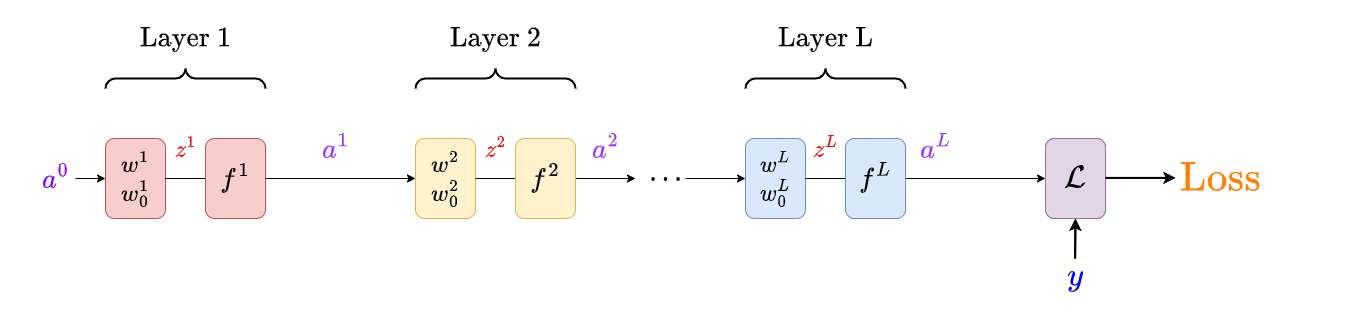
\includegraphics[width=180mm,scale=0.4]{images/nn_1_5_images/network_bp.png}
        \end{figure}
        
        This may look intimidating, but we already have all the tools we need to handle this problem.
        
        Our goal is to get a \textbf{gradient} for each of our \textbf{weight} vectors $w^\ell$, so we can do gradient descent and \textbf{improve} our model.
        
        According to our above analysis in Concept 9, we need only a few steps to get all of our gradients.
        
        \begin{concept}
            In order to do \vocab{back-propagation}, we have to build up our \vocab{chain rule} for each weight gradient.
            
            \begin{itemize}
                \item We start our chain rule with one term shared by every gradient: 
                    \begin{equation*}
                        \overbrace{
                            \pderiv {\pur{\loss}} {\blu{a^L}} 
                        }^{\text{Loss unit}}
                    \end{equation*}
            \end{itemize}
            
            Then, we follow these two steps until we run out of layers:
            \begin{itemize}
                \item We're at layer $\ell$. We want to get the \purp{weight gradient} for this layer. We get this by \gren{multiplying} our chain rule by
                
                    \begin{equation*}
                        \overbrace{
                            \pderiv {\blu{a^\ell}} {\red{z^\ell}}
                        }^{\text{Within layer}}
                            \cmul
                        \overbrace{
                            \pderiv {\red{z^\ell}} {w^\ell}
                        }^{\text{Get weight grad}}
                    \end{equation*}
                    
                    We \red{exclude} this term for any other gradients we want.
                
                \item If we aren't at layer 1, there's a previous layer we want to get the weight for. We reach layer $\ell-1$ by multiplying our chain rule by 
                
                    \begin{equation*}
                        \overbrace{
                            \pderiv {\blu{a^\ell}} {\red{z^\ell}}
                        }^{\text{Within layer}}
                            \cmul
                        \overbrace{
                            \pderiv {\red{z^\ell}} {a^{\ell-1}}
                        }^{\text{Link layers}}
                    \end{equation*}
            \end{itemize}
            
            Once we reach layer 1, we have \gren{every single} weight vector we need! Repeat the process for $w_0$ gradients and then do \purp{gradient descent}.
        \end{concept}
        
        Let's get an idea of what this looks like in general:
        
        \begin{equation}
            \pderiv {\pur{\loss}} {w^\ell} 
            =
            \overbrace{
                \Bigg(
                    \pderiv {\pur{\loss}} {\blu{a^L}} 
                \Bigg)
            }^{\text{Loss unit}}
            \cmul
            \overbrace{
                \Bigg(
                    \pderiv {\blu{a^L}}   {\red{z^L}}
                        \cmul
                    \pderiv {\red{z^L}}   {a^{L-1}}
                \Bigg) 
            }^{\text{Layer $L$}}
            \cmul
            \overbrace{
                \Bigg(
                    \pderiv {\blu{a^{L-1}}}   {\red{z^{L-1}}}
                        \cmul
                    \pderiv {\red{z^{L-1}}}   {a^{L-2}}
                \Bigg) 
            }^{\text{Layer $L-1$}}
            \cmul
            \Bigg(
                \cdots 
            \Bigg)
            \cmul
            \overbrace{
                \Bigg(
                    \pderiv {\blu{a^\ell}}   {\red{z^\ell}}
                        \cmul
                    \pderiv {\red{z^\ell}}   {w^{\ell}}
                \Bigg) 
            }^{\text{Layer $\ell$}}
        \end{equation}
        
        That's pretty ugly. If we need to hide the complexity, we can:\\
        
        \begin{notation}
            If you need to do so for \purp{ease}, you can \vocab{compress}  your \vocab{derivatives}. For example, if we want to only have the last weight term \gren{separate}, we can do:
            
            \begin{equation}
                \pderiv {\pur{\loss}} {w^\ell} 
                =
                \overbrace{
                    \pderiv {\pur{\loss}} {\red{z^\ell}} 
                }^{\text{Other}}
                \cmul
                \overbrace{
                    \pderiv {\red{z^\ell}}   {w^\ell}
                }^{\text{Weight term}}
            \end{equation}
        \end{notation}
        
        But we should also explore what each of these terms \textit{are}.
        